\documentclass[a4paper,12pt]{article}

% --- Essential Packages ---
\usepackage[utf8]{inputenc}
\usepackage[T1]{fontenc}
\usepackage[english]{babel}
\usepackage{geometry}
\usepackage{graphicx}
\usepackage{hyperref}
\usepackage{listings}
\usepackage{xcolor}
\usepackage{float}
\usepackage{fancyhdr}
\usepackage{titlesec}
\usepackage{enumitem}
\usepackage{booktabs}
\usepackage{parskip}
\usepackage{tikz}
\usepackage{pgfplots}
\pgfplotsset{compat=1.18}

% --- Page Configuration ---
\geometry{margin=2.5cm, top=3cm, bottom=3cm}

% --- Color Scheme ---
\definecolor{codegray}{gray}{0.95}

% --- Hyperlink Configuration ---
\hypersetup{
    colorlinks=true,
    linkcolor=black,
    urlcolor=black,
    citecolor=black,
    pdftitle={Technical Report - Concurrent HTTP Web Server},
    pdfauthor={Martim Gil, Nuno Leite Faria}
}

% --- Code Style ---
\lstset{
    backgroundcolor=\color{codegray},
    basicstyle=\ttfamily\small,
    breaklines=true,
    frame=single,
    framerule=0.5pt,
    rulecolor=\color{black},
    numbers=left,
    numberstyle=\tiny,
    captionpos=b,
    keywordstyle=\bfseries,
    commentstyle=\itshape,
    stringstyle=\ttfamily,
    showstringspaces=false,
    tabsize=4,
    xleftmargin=1em,
    xrightmargin=1em,
    aboveskip=1em,
    belowskip=1em,
    language=C
}

% --- Header and Footer ---
\setlength{\headheight}{14pt}
\pagestyle{fancy}
\fancyhf{}
\fancyhead[L]{\small\textit{Concurrent HTTP Web Server}}
\fancyhead[R]{\small\textit{Technical Report}}
\fancyfoot[C]{\thepage}
\renewcommand{\headrulewidth}{0.4pt}
\renewcommand{\footrulewidth}{0pt}

% --- Section Styling ---
\titleformat{\section}{\Large\bfseries}{\thesection}{1em}{}
\titleformat{\subsection}{\large\bfseries}{\thesubsection}{1em}{}
\titleformat{\subsubsection}{\normalsize\bfseries}{\thesubsubsection}{1em}{}

% --- List Styling ---
\setlist[itemize]{noitemsep, topsep=0.5em}
\setlist[enumerate]{noitemsep, topsep=0.5em}

\begin{document}

% =================================================================
% TITLE PAGE
% =================================================================
\begin{titlepage}
    \centering
    
    % --- DETI Logo ---
    \vspace*{2cm}
    \includegraphics[width=0.7\textwidth]{deti.png}
    
    \vspace{3cm}
    
    % --- Document Title ---
    {\Huge\textbf{Technical Report}}\\[0.5cm]
    {\LARGE Concurrent HTTP Web Server}
    
    \vspace{1.5cm}
    
    % --- Decorative Line ---
    \rule{0.6\textwidth}{0.5pt}
    
    \vspace{1.5cm}
    
    % --- Course Information ---
    {\Large\textbf{Operating Systems}}\\[0.3cm]
    {\large Academic Year 2024/2025}
    
    \vspace{2cm}
    
    % --- Authors ---
    \begin{tabular}{cc}
        \textbf{Martim Gil} & \textbf{Nuno Leite Faria} \\
        Student ID: 124833 & Student ID: 112994 \\
    \end{tabular}
    
    \vspace{1.5cm}
    
    % --- Supervisor ---
    {\large Supervisor: Prof. Pedro Azevedo Fernandes}
    
    \vfill
    
    % --- Date ---
    {\large \today}
    
\end{titlepage}

% --- Abstract ---
\begin{abstract}
This document details the development of a concurrent HTTP server built in C for the Operating Systems course at the University of Aveiro.

The main goal of the project was to build a system capable of manage numerous client requests at the same time using a combined process–thread architecture.

The system utilizes synchronization and interprocess communication methods, particulary POSIX semaphores and shared memory. These elements ensure consistency and mutual exclusion during access to shared resources. 
Extra modules were added for safe concurrent logging, file caching, and live statistics tracking.

The results highlight the system's reliability, scalability, and precision in synchronization mechanisms, as well as its stable performance even under heavy workloads.
\end{abstract}

% --- Table of Contents ---
\tableofcontents
\newpage

% ----------------------------------------------------------------------
% 1. Introduction
% ----------------------------------------------------------------------
\section{Introduction}

Building concurrent servers stands the most effective and demonstrative uses of synchronization, inter-process communication, and thread management concepts explored in operating systems.

This project aimed to deploy a effective HTTP server that can handle multiple concurrent client requests at the same time.

The C programming language was used, utilizing POSIX system calls for thread creation and synchronization, semaphore management, shared memory management, and inter-process communication. 
The architecture of the system is modularly designed, ensuring that various components are easy to maintain and extend.

% ----------------------------------------------------------------------
% 2. Implementation Details
% ----------------------------------------------------------------------
\section{Implementation Details}

The implementation have a modular architecture in which each subsystem is represented by a dedicated source file or pair of header and implementation files under the \texttt{src/} directory.  

This structure enhances reusability, maintainability, and clear separation of concerns between the networking layer, synchronization mechanisms, and data management components.

The Diagram below shows the structure:

\begin{itemize}
  \item \textbf{concurrent-http-server/} (root directory)
  \begin{itemize}
    \item .gitignore
    \item Makefile
    \item README.md
    \item server.conf
    \item server.log, access.log
    \item \textbf{docs/} - Documentation and reports
    \begin{itemize}
      \item design/ - LaTeX design document
      \item report/ - Technical report (LaTeX + PDF)
      \item user\_manual/ - End-user manual
    \end{itemize}
    \item \textbf{enunciados/} - Documentation given as project guidelines
    \item \textbf{src/} - All C source code (core of the system)
    \begin{itemize}
      \item cache.c, cache.h
      \item config.c, config.h
      \item http\_builder.c, http\_builder.h
      \item http\_parser.c, http\_parser.h
      \item logger.c, logger.h
      \item master.c
      \item semaphores.c, semaphores.h
      \item shared\_mem.c, shared\_mem.h
      \item stats.c, stats.h
      \item stats\_reader.c
      \item thread\_logger.c
      \item thread\_pool.c, thread\_pool.h
      \item worker.c, worker.h
    \end{itemize}
    \item \textbf{tests/} - Automated and manual testing scripts
    \begin{itemize}
      \item README.md
      \item stress\_test.sh
      \item test\_concurrent.c
      \item stress\_client.c
      \item test\_suite.sh
    \end{itemize}
    \item \textbf{www/} - Static web content served by the HTTP server
    \begin{itemize}
      \item dashboard.html - Real-time statistics dashboard (Bonus Feature)
      \item index.html, style.css, script.js, script.ts
      \item image.png, doc.pdf
      \item images/ - Image assets directory
      \item errors/ - Error pages (404.html, 500.html)
    \end{itemize}
    \item \textbf{bin/} - Generated during compilation (created by Makefile)
    \begin{itemize}
      \item webserver (compiled binary)
    \end{itemize}
  \end{itemize}
\end{itemize}


\subsection{System Architecture}

This project is made of three main execution entities: the \textbf{master process}, the \textbf{worker processes}, and the \textbf{auxiliary tools}.  
The master process is responsible for system initialization, socket setup, configuration parsing, coordination of shared resources, and forking worker processes.  
Each worker process maintains its own thread pool, where individual threads handle client connections concurrently.  
Auxiliary programs, such as \texttt{stats\_reader}, interact with the server's shared memory region to show runtime statistics without interfering with normal operation.

The core modules are summarized below:

\begin{itemize}
  \item \textbf{master.c} – Initializes the system, loads configuration parameters, creates synchronization primitives, and launches the listening socket. It also spawns the thread pool and dispatches incoming connections.
  \item \textbf{worker.c / worker.h} – Implements the logic executed by each worker thread. It reads HTTP requests, interacts with the cache and statistics modules, and builds HTTP responses.
  \item \textbf{thread\_pool.c / .h} – Manages a fixed number of worker threads and a queue of pending tasks. This module is responsible for dynamic workload distribution and concurrency control.
  \item \textbf{cache.c / .h} – Provides an in-memory file cache to reduce disk I/O. Cached entries are protected by semaphores to ensure mutual exclusion.
  \item \textbf{logger.c / .h} and \textbf{thread\_logger.c} – Implement thread-safe logging using semaphores to serialize write operations to the log file.
  \item \textbf{stats.c / .h} and \textbf{shared\_mem.c / .h} – Manage global statistics (requests, bytes, cache hits) stored in a POSIX shared memory region accessible from the external reader program.
  \item \textbf{semaphores.c / .h} – Encapsulates POSIX semaphore operations (\texttt{sem\_open}, \texttt{sem\_wait}, \texttt{sem\_post}, etc.) to provide a clean synchronization interface.
  \item \textbf{http\_parser.c / .h} and \textbf{http\_builder.c / .h} – Handle HTTP protocol parsing and response construction.
  \item \textbf{config.c / .h} – Loads server parameters such as port, document root, cache size, and number of threads from \texttt{server.conf}.
\end{itemize}

\subsection{Process and Thread Management}
The concurrent HTTP server uses a combined process–thread architecture that separates the acceptance of client connections from the handling of individual requests.  
The \texttt{master} process is responsible for system initialization, resource allocation, and the creation of a fixed-size thread pool.  
This approach avoids the overhead associated with creating and destroying threads on demand while allowing high levels of concurrency and efficient resource utilization.

Once the server started, the \texttt{master} process enters a blocking loop where it can accepts incoming TCP connections through the listening socket.  
For each connection that is accepted, the corresponding file descriptor is packaged as a task and submitted to the thread pool by invoking the function \texttt{thread\_pool\_add\_task()}.  

\paragraph{Thread Pool Initialization.}
The thread pool, located in \texttt{src/thread\_pool.c}, is initialized with a fixed number of worker threads determined by the configuration file (\texttt{server.conf}).  
Each thread is created at startup using the POSIX \texttt{pthread\_create()} function and executes a continuous loop defined in the \texttt{thread\_worker()}.  
At the start, all threads enter a waiting state, blocked on a condition variable until new work becomes available in the shared task queue.

\paragraph{Task Scheduling.}

Tasks are kept in a synchronized queue secured by a mutex. When the master process adds a new connection to the queue, it maintain the queue and places the socket descriptor, and notifies one of the waiting threads by calling \texttt{pthread\_cond\_signal()}.
When the signal is received, a worker thread activates, find the task, and frees the mutex, and starts handling the connection. 
If there are no tasks present, threads stay idle, blocked on the condition variable.


\paragraph{Worker Thread Execution.}
Every worker thread, found in \texttt{src/worker.c}, is accountable for managing an individual HTTP transaction. The workflow for execution is the following:

\begin{enumerate}
  \item Obtain the HTTP request from the designated socket descriptor.
  \item Analyze the request with the \texttt{http\_parser} to obtain the method, path, and headings.
  \item Check if the requested resource is present in the cache. If it isn't available, get it back from the disk and place it into the cache.
  \item Construct the HTTP response utilizing the \texttt{http\_builder} and return it to the client.
  \item Revise the common statistics stored in memory (e.g., total requests, cache hits/misses) and add an entry to the log.
\end{enumerate}

This structure enables several worker threads to function simultaneously on different connections while the access to common resources like the cache, statistics counters, and log files—stays coordinated through semaphores and mutexes

\paragraph{Synchronization and Graceful Shutdown.}
The use of condition variables guarantees efficient coordination between the master process and worker threads.  
During server shutdown, the master process signals all condition variables, allowing blocked threads to exit their waiting loops.  
Each thread is then joined using \texttt{pthread\_join()}, assuring a clean and orderly release of all allocated resources.

Overall, the process and thread management strategy balances concurrency with control, providing scalable performance while maintaining thread safety and predictability in the server’s behavior.

\subsection{Synchronization and IPC}
To have a reliable and consistent operation in a multithreaded setting, the server uses synchronization methods utilizing POSIX semaphores, mutexes, and shared memory. 
This safeguard common resources like the task queue, the cache, the data, and the log file.



\paragraph{Semaphore Abstraction.}
The semaphore subsystem encapsulates the POSIX API functions \texttt{sem\_open()}, \texttt{sem\_wait()}, \texttt{sem\_post()}, and \texttt{sem\_unlink()}, offering operations such as \texttt{semCreate()}, \texttt{semConnect()}, \texttt{semDown()}, and \texttt{semUp()}.  
Each semaphore is initialized with an initial value depending on its purpose (e.g., binary for mutual exclusion, counting for producer--consumer synchronization).  

\paragraph{Producer--Consumer Coordination.}
The interaction between the master process and the worker threads follows the producer--consumer model.  
The master acts as the producer by inserting new tasks (socket descriptors) into a shared circular buffer implemented in the thread pool, while the workers act as consumers by retrieving and processing these tasks.  
Access to the buffer is controlled by two semaphores:
\begin{itemize}
  \item A \emph{counting semaphore} representing the number of available tasks.
  \item A \emph{binary semaphore} (mutex) protecting concurrent access to the queue structure itself.
\end{itemize}

\paragraph{Shared Statistics and Atomicity.}
Global runtime metrics, including total requests served, bytes transmitted, and cache hit/miss counters, are stored in a POSIX shared memory region managed by \texttt{src/shared\_mem.c}.  
All accesses are wrapped in critical sections protected by binary semaphores.  
This ensures atomicity of operations such as:
\begin{verbatim}
stats.requests++;
stats.bytes_sent += response_size;
\end{verbatim}
The external utility \texttt{stats\_reader} connects to the same shared memory object and can read these values in real time.

\paragraph{Mutual Exclusion in Shared Logging.}
Logging operations, implemented in \texttt{src/logger.c} and \texttt{src/thread\_logger.c}, are performed concurrently by multiple worker threads.  
To prevent simultaneous writes that could corrupt the log file, a named binary semaphore ensures exclusive access to the output stream.  
When a thread intends to log an event, it performs a \texttt{semDown()} operation before writing and a \texttt{semUp()} afterward.

\paragraph{Synchronization Robustness.}
Using named semaphores and shared memory, the system allows independent processes to coordinate while maintaining persistence across program instances.  
All synchronization objects are unlinked and destroyed at shutdown, ensuring that no orphaned semaphores or shared memory regions remain active.  
This make sure that we have a reliable and consistent cleanup and prevents resource leakage in the operating system.


\subsection{Resource Management (Cache and Files)}
% Explain LRU Cache algorithm.
% Use of Reader-Writer Locks (pthread_rwlock) for performance.
% Reference: src/cache.c
The system uses in-memory caching mechanism implemented in \texttt{src/cache.c}.  
The cache temporarily stores the contents of frequently requested files, allowing subsequent requests for the same resource to be served directly from memory without accessing the filesystem.

\paragraph{Cache Architecture.}
The cache is implemented as a fixed-size table of entries, each representing a single cached file.  
Each entry stores the following attributes:
\begin{itemize}
  \item The file path (\texttt{char *path});
  \item A pointer to the file content loaded into memory;
  \item The file size (in bytes);
  \item Metadata for cache management, such as last access time or usage counter.
\end{itemize}
The total number of entries and the maximum memory size are defined in the configuration file (\texttt{server.conf}) and initialized at server startup by the \texttt{cache\_init()}.

\paragraph{LRU Replacement Policy.}
When the cache becomes fully populated, it needs to remove an current entry to allow for new information. The executed plan follows the \textbf{Least Recently Used (LRU)} strategy, which removes the entry that has not been accessed, for an extended period. Every cache entry keeps a timestamp that gets refreshed with each entry. 
Upon adding, the system loops through the cache table to find the least just utilized the current entry and substitutes it with the updated file information. 

\paragraph{Reader--Writer Locking.}
To support concurrent read and write operations on the cache, the implementation employs \textbf{POSIX reader–writer locks} (\texttt{pthread\_rwlock\_t}).  
These locks allow multiple worker threads to read cache entries simultaneously, while ensuring that write operations (such as file insertion or eviction) occur exclusively.  
The concurrency model operates as follows:
\begin{itemize}
  \item \textbf{Readers (cache hits):} When a requested file is present in the cache, the worker thread obtains a \emph{read lock} (\texttt{pthread\_rwlock\_rdlock()}) to access the entry without obstructing other readers.
  \item \textbf{Writers (cache misses or evictions):} When a file needs to be added or modified, the thread obtains a \emph{write lock} (\texttt{pthread\_rwlock\_wrlock()}) to make sure it's the only one access, blocking any concurrent reads or writes.
\end{itemize}

\paragraph{File Loading and Caching Workflow.}
When a worker thread handles a client after receiving the request, it checks the cache through \texttt{cache\_lookup(path)}. If the file is located (cache hit), the data is instantly transmitted to the client. 
If the document isn't stored in the cache (cache miss), this actions take place:
\begin{enumerate}
  \item The thread acquires a write lock to ensure exclusive access.
  \item The file is opened from the disk using standard I/O routines (\texttt{open()}, \texttt{read()}, \texttt{stat()}).
  \item The file content is copied into allocated memory and stored in a cache slot.
  \item The cache metadata (timestamp, size) is updated, and the lock is released.
\end{enumerate}

\paragraph{Cache Coherency and Statistics.}
Every access to the cache updates its usage metadata and increments the corresponding statistics counters for \emph{cache hits} and \emph{cache misses}, managed by \texttt{src/stats.c}.  
These counters uses semaphores to have atomicity and can be viewed in real time through the \texttt{stats\_reader} utility.  
By combining semaphores for atomic counters and reader–writer locks for cache access, the implementation achieves both correctness and high throughput.

\paragraph{Resource Cleanup.}
At shutdown, the cache is fully cleared by the \texttt{cache\_destroy()}, which iterates over all valid entries, frees allocated memory buffers, and releases synchronization primitives.  
This prevents memory leaks and ensures that all file descriptors and dynamically allocated structures are properly deallocated before process termination.

\subsection{HTTP Processing}
% Request parsing and response construction.
% Error handling (404, 403, 500).
% Reference: src/http_parser.c, src/http_builder.c
The HTTP layer is responsible for interpreting client requests and generating
valid responses. It is implemented through two core modules:
\texttt{http\_parser.c} and \texttt{http\_builder.c}, which together handle
message parsing, header construction, and delivery to the client socket.

\paragraph{Request Handling.}
Each worker thread receives raw data from the client socket and invokes the parser to
extract the method, resource path, and protocol version. Optional headers such as
\texttt{Range} are also recognized, enabling support for partial content delivery.
The parser performs minimal tokenization and boundary validation, storing the
result in a compact structure that represents the parsed request. Invalid or malformed
requests trigger a direct \texttt{400 Bad Request} response.

\paragraph{Response Generation.}
Once a request has been validated and the corresponding file located (either from
cache or disk), the builder module assembles the complete HTTP response. This includes
the status line, headers such as \texttt{Content-Type}, \texttt{Content-Length},
and \texttt{Connection}, and the optional body. Specialized routines also support
partial responses for range requests, enabling clients to resume interrupted
downloads. Responses are sent directly through the socket using formatted writes
to ensure efficient transmission.

\paragraph{Error Responses.}
For failed operations, such as missing files or internal I/O errors, the server emits
concise HTML error pages with status codes \texttt{404} or \texttt{500}. These are
generated dynamically using a standard template, ensuring consistent presentation
across error types.

\paragraph{Performance and Extensibility.}
The separation between request parsing and response construction ensures a clear
processing pipeline, minimizing contention and simplifying maintenance. This modular
design supports high throughput under concurrent workloads and can be easily extended
to accommodate new request types, caching strategies, or content-handling features
without altering the core logic of the server.

\subsection{Implemented Bonus Features}

The server implements three additional features.

\subsubsection{Real-time Web Dashboard}
A monitoring page is accessible at \texttt{/dashboard.html}.
\begin{itemize}
    \item \textbf{Backend:} A dedicated API endpoint (\texttt{/api/stats}) was created. Unlike standard file requests, this endpoint bypasses the disk cache and reads directly from the global \texttt{server\_stats\_t} structure in POSIX Shared Memory. 
    \item \textbf{Frontend:} A responsive HTML and JavaScript interface polls this API asynchronously every 2 seconds, rendering live charts of throughput, latency, and cache efficiency without requiring a page reload. We also used Tailwind CSS and Shadcn UI.
\end{itemize}

\subsubsection{HTTP Keep-Alive}
The server supports persistent connections, controlled by the \texttt{TIMEOUT\_SECONDS} parameter in \texttt{server.conf}.
\begin{itemize}
    \item Instead of closing the TCP socket immediately after a response, the worker thread keeps the connection open, waiting for subsequent requests from the same client.
\end{itemize}

\subsubsection{Range Requests / Partial Content}
To support media streaming and download resumption, the server implements \texttt{HTTP 206 Partial Content}.
\begin{itemize}
    \item The HTTP parser detects the \texttt{Range: bytes=x-y} header.
    \item The file reader uses \texttt{fseek()} to jump to the requested offset and serves only the specific byte chunk.
    \item The builder constructs the appropriate \texttt{Content-Range} header, allowing clients (like video players) to buffer content efficiently.
\end{itemize}

% ----------------------------------------------------------------------
% 3. Challenges and Solutions
% ----------------------------------------------------------------------
\section{Challenges and Solutions}
% Critical section to show understanding of concurrency issues.
The development of a concurrent HTTP server presented several challenges related to synchronization and interprocess communication.
Designing a program with thread-safety and with data consistency, while making use of proper cleanup and resource management in all executable scenarios.
Because of this, this section aims to bring light to what were considered the key obstacles in the implementation of the solution we provided.

\subsection{Race Conditions}
% Example: "We detected statistics were losing counts..."
% Solution: "Implemented an exclusive semaphore for the stats struct."
During the early stages of development, one of the most difficult concurrency issues encountered was the presence of \textbf{race conditions} in the shared statistics subsystem.  
The \texttt{stats} structure, stored in a shared memory region, was updated concurrently by multiple worker threads each time a request was served.  
Because these updates occurred without proper synchronization, simultaneous increments of counters such as \texttt{requests} and \texttt{bytes\_sent} overwrote each other’s values, resulting in lost counts and wrong statistics.

\paragraph{Problem Observation.}
The issue during stress testing, where the total number of processed requests reported by \texttt{stats\_reader} was consistently lower than the number of actual HTTP requests completed by the server.  
This confirmed that concurrent updates to the same memory region were not atomic and were being interrupted by other threads before completion.

\paragraph{Solution.}
To ensure atomicity, an \textbf{exclusive binary semaphore} was introduced to protect all accesses to the shared \texttt{stats} structure.  
Before any modification, a worker thread performs a \texttt{semDown()} operation to acquire exclusive access, updates the relevant counters, and then releases the lock with \texttt{semUp()}.  
This mechanism guarantees that only one thread at a time can modify the shared statistics, effectively eliminating data races and lost updates.

\paragraph{Verification.}
After the introduction of this semaphore, repeated executions of the \texttt{test\_concurrent.c} and \texttt{stress\_test.sh} scripts produced consistent results:  
the total request count reported by \texttt{stats\_reader} matched the number of served HTTP responses.  
This confirmed that the synchronization strategy successfully enforced atomicity and consistency of shared statistical data across all worker threads.

\subsection{Memory Management and Leaks}
% Discussion on Valgrind usage.
% Ensuring shared memory is cleaned (unlink) on shutdown (SIGINT).
Memory management played a crucial role in the reliability and robustness of the server.  
Because the system relies on dynamic memory allocation, shared memory segments, and synchronization primitives created at runtime, any mismanagement could result in resource leaks or instability after repeated executions.

\paragraph{Leak Detection with Valgrind.}
Throughout the development, the \textbf{Valgrind} analysis tool was used to detect and diagnose memory leaks, invalid reads or writes, and unfreed heap allocations.  
Running the server under Valgrind with realistic workloads revealed a small number of unreleased buffers within the cache subsystem and unclosed file descriptors associated with the logging mechanism.  
These issues were corrected by guarantee that all dynamically allocated buffers are freed, all open files are closed, and all synchronization primitives are properly destroyed before process termination.

\paragraph{Shared Memory and Semaphore Cleanup.}
The server makes use of POSIX shared memory objects and named semaphores to enable interprocess communication between the main server and auxiliary tools such as \texttt{stats\_reader}.  
Improper shutdown or unexpected termination (\texttt{Ctrl+C}) initially left behind orphaned resources that persisted in the system, visible through \texttt{ipcs} or \texttt{ls /dev/shm}.  
To address this, explicit cleanup routines were implemented in \texttt{src/shared\_mem.c} and \texttt{src/semaphores.c}.  
These routines perform the following actions:
\begin{itemize}
  \item Unlink all named semaphores using \texttt{sem\_unlink()};
  \item Unmap and close the shared memory segment via \texttt{munmap()} and \texttt{shm\_unlink()};
  \item Free dynamically allocated memory structures associated with cache entries and statistics.
\end{itemize}

\paragraph{Signal-Driven Resource Management.}
To guarantee cleanup even in the case of user interruption, the master process installs custom signal handlers for \texttt{SIGINT} and \texttt{SIGTERM}.  
When triggered, these handlers invoke a global \texttt{cleanup()} function that sequentially joins all worker threads, destroys synchronization objects, releases cache memory, and removes shared memory objects from the system.  
This ensures a graceful shutdown sequence, preventing resource leakage even under abrupt termination scenarios.

\paragraph{Verification and Stability.}
After the integration of the cleanup logic, repeated Valgrind analyses confirmed that all heap allocations were correctly released, with the final summary reporting:
\begin{verbatim}
== All heap blocks were freed -- no leaks are possible ==
\end{verbatim}
Additionally, post-execution checks using \texttt{ipcs -m} and \texttt{ipcs -s} verified that no shared memory segments or semaphores remained active after server shutdown.  


\subsection{Log Synchronization}
% The problem of interleaved log lines.
% Implemented solution (local buffer or mutex).
Another challenge was the occurrence of interleaved log entries in the system log file, because of multiple worker threads perform logging operations simultaneously, concurrent calls to \texttt{fprintf()} resulted in overlapping text output, corrupted lines, or partial messages, making debugging difficult.

\paragraph{Problem Analysis.}
The logging subsystem, implemented in \texttt{src/logger.c}, originally allowed each worker thread to write directly to the shared log file without synchronization.  
During concurrent request handling, multiple threads invoked \texttt{logger\_write()} simultaneously, causing their respective I/O streams to interfere.  
Since standard C file I/O is not inherently atomic, different threads could write portions of separate log entries into the same buffer region, producing output such as:
\begin{verbatim}
[Thread 2] Served file index.html [Thread 3] Client disconnected
[Thread 5] Serv[Thread 4] Error 404: file not found
\end{verbatim}
This problem not only compromised readability but also impeded accurate debugging and event tracing.

\paragraph{Implemented Solution.}
To ensure the integrity of log entries, a mutual exclusion mechanism was introduced around all file-writing operations.  
A \emph{binary semaphore} named \texttt{/ws\_log\_sem} is created during server initialization and shared among all threads.  
Whenever a worker intends to write to the log, it executes a \texttt{semDown()} (wait) operation before writing and a \texttt{semUp()} (post) operation afterward, guaranteeing exclusive access to the log stream during the write.

In addition, the \texttt{src/thread\_logger.c} module provides each thread with a small local buffer used to assemble the entire log message before issuing a single, atomic write operation to the shared file.  
This design minimizes the duration of critical sections and reduces contention between threads.

\paragraph{Example Implementation.}
The final logging sequence for each worker thread is as follows:
\begin{enumerate}
  \item Format the log message locally using \texttt{snprintf()} into a thread-local buffer.
  \item Acquire the global logging semaphore using \texttt{semDown()}.
  \item Write the buffered message to the log file using \texttt{fprintf()} or \texttt{write()}.
  \item Flush the stream with \texttt{fflush()} to ensure persistence.
  \item Release the semaphore using \texttt{semUp()}.
\end{enumerate}
This ensures that only one thread writes to the file at a time and that each log entry is complete.

\paragraph{Verification.}
Following the implementation of the synchronization mechanism, repeated stress tests involving dozens of concurrent clients confirmed that all log entries were well-formed, non-overlapping, and timestamped correctly.  
Furthermore, log inspection tools and diff comparisons across multiple runs revealed identical, reproducible outputs under equivalent workloads, validating that the synchronization scheme effectively eliminated race conditions in the logging subsystem.

\subsection{Zombies and Signals}
% How SIGCHLD or waitpid was handled in Master to prevent zombies.
During development, one critical aspect of maintaining process hygiene in the server was the prevention of zombie processes.  
A zombie process occurs when a child process terminates but its exit status remains uncollected by the parent, leaving a defunct entry in the system’s process table.  
Although the concurrent HTTP server primarily relies on threads for parallelism, auxiliary processes such as the master and worker components, or other spawned utilities, can still generate zombies if not properly reaped.

\paragraph{Problem Description.}
Test executions revealed lingering defunct processes after multiple start-and-stop cycles of the server.  
Inspection using the \texttt{ps -ef} and \texttt{top} commands showed entries in the \emph{Z} (zombie) state, indicating that terminated child processes had not been reaped by the master.  
This occurred because no signal handler was initially configured to capture \texttt{SIGCHLD}, the signal sent to a parent when one of its children exits.

\paragraph{Implemented Solution.}
To address the accumulation of zombie processes, a dedicated signal handler for \texttt{SIGCHLD} was registered in the master process (see \texttt{src/master.c}).  
This handler performs a non-blocking call to \texttt{waitpid()} with the \texttt{WNOHANG} option, which immediately reaps any terminated child processes without interrupting the server’s main accept loop.  
The implementation follows tis:

\begin{verbatim}
void sigchld_handler(int signo) {
    while (waitpid(-1, NULL, WNOHANG) > 0);
}
\end{verbatim}

This ensures that all child processes are properly cleaned up as soon as they terminate, preventing accumulation of zombies.

\paragraph{Graceful Shutdown Signals.}
In addition to \texttt{SIGCHLD}, the master process also handles \texttt{SIGINT} and \texttt{SIGTERM} to ensure graceful server termination.  
When either of these signals is received, the signal handler triggers a global cleanup routine that:
\begin{itemize}
  \item Closes all open sockets and joins all worker threads.
  \item Releases semaphores and shared memory objects.
  \item Calls \texttt{logger\_close()} and \texttt{cache\_destroy()} to release I/O and heap resources.
\end{itemize}
By installing these handlers during initialization, the server guarantees that abrupt termination via keyboard interrupt (\texttt{Ctrl+C}) or system kill command results in full resource cleanup.

\paragraph{Verification.}
To confirm correct signal handling and zombie prevention, repeated executions of the server under heavy load were followed by process table inspection using:
\begin{verbatim}
$ ps -ef | grep server
\end{verbatim}
No processes in the \texttt{Z} (zombie) state were observed after shutdown, and the system returned all allocated process slots to the system immediately.  
These results demonstrate that the combination of \texttt{SIGCHLD} reaping and structured termination handlers effectively eliminates zombie processes and the cleanup process.

% ----------------------------------------------------------------------
% 4. Testing Methodology
% ----------------------------------------------------------------------
\section{Testing Methodology}
% Describe how the server was validated.
% Mention 'test_suite.sh' and 'test_concurrent.c'.
The validation of the concurrent HTTP server was performed through a structured testing framework combining automated functional validation, concurrency stress testing, and static and dynamic analysis tools.  
Testing focused on ensuring that the system correctly implemented HTTP semantics, handled concurrent requests safely, and maintained stability under heavy load conditions.

\subsection{Functional Tests}
% curl, mime-type validation, status codes.
Functional verification was carried out using a series of automated shell scripts and manual HTTP inspections.  
The main script, \texttt{tests/test\_suite.sh}, executes  routines that compile the server, launch it in a environment, and issue a predefined set of HTTP requests using the \texttt{curl} utility.

\paragraph{HTTP Response Validation.}
Each request is checked:
\begin{itemize}
  \item Correct HTTP status codes: \texttt{200 OK}, \texttt{404 Not Found}, and \texttt{500 Internal Server Error}.
  \item Accurate \texttt{Content-Length} and \texttt{Content-Type} (MIME type) headers.
  \item Proper file serving from the \texttt{www/} directory and custom error pages from \texttt{www/errors/}.
\end{itemize}
The tests also covers malformed or non-existent URLs to ensure the server’s error-handling path responds.

\paragraph{Automated Makefile Integration.}
The testing scripts are directly integrated into the project’s \texttt{Makefile} through the targets:
\begin{verbatim}
make test       # Execute functional validation via test_suite.sh
\end{verbatim}

\paragraph{Verification of MIME Type Handling.}
To ensure that different file types were correctly served, the server’s response headers were compared against expected MIME types defined by the \texttt{http\_builder.c} module.  
For instance, \texttt{.html}, \texttt{.css}, and \texttt{.png} files were validated to produce \texttt{text/html}, \texttt{text/css}, and \texttt{image/png} respectively.  

\paragraph{Result Summary.}
All functional tests passed, confirming proper routing of static files, reliable handling of error responses, and complete protocol compliance.  
Log inspection confirmed that each request generated a corresponding, timestamped entry without corruption or duplication.


\subsection{Concurrency and Stress Tests}
% Usage of Apache Bench (ab).
% Validation with Helgrind/ThreadSanitizer (TSan).
To validate synchronization correctness and scalability, we included both native and external concurrency testing tools.  
Our goal was to ensure that multiple simultaneous clients could interact with the server without introducing race conditions, deadlocks, or resource starvation.

\paragraph{Automated Concurrency Validation.}
The \texttt{tests/test\_concurrent.c} program was developed to create a controlled, reproducible concurrency test harness.  
It spawns multiple client threads that simultaneously perform HTTP requests, validating that:

\begin{itemize}
  \item No request data is lost or partially transmitted.
  \item Response latency remains stable under load.
  \item Shared statistics and cache metrics remain consistent across threads.
\end{itemize}


\paragraph{Load Testing with Apache Bench.}
In addition to internal tools, we used ApacheBench (ab) to simulate large-scale traffic.  
Typical test commands included:

\begin{verbatim}
ab -n 500 -c 50 http://localhost:8080/index.html
\end{verbatim}

where \texttt{-n} specifies the total number of requests and \texttt{-c} the concurrency level.  
Metrics such as average request latency, throughput, and connection error rate were recorded.  
The server demonstrated stable throughput and no data corruption even beyond 100 concurrent requests.

\paragraph{Race Detection with Helgrind and ThreadSanitizer.}
Dynamic analysis was further strengthened using \textbf{Helgrind} (a Valgrind tool) and \textbf{ThreadSanitizer (TSan)} to detect hidden race conditions in the multithreaded subsystems.  
Running the server under these tools we verified that:
\begin{itemize}
  \item No concurrent data races occurred within the cache, logger, or statistics modules.
  \item All synchronization primitives (mutexes, semaphores, and reader–writer locks) were properly initialized and destroyed.
  \item Condition variables and thread joins were correctly paired, avoiding deadlocks or missed signals.
\end{itemize}

\paragraph{Stress and Stability Evaluation.}
The \texttt{tests/stress\_test.sh} script launched high-frequency, randomized HTTP requests against the server for extended durations.  
Monitoring through the \texttt{stats\_reader} utility confirmed steady-state operation, with no memory leaks or semaphore exhaustion observed during multi-minute runs.

% ----------------------------------------------------------------------
% 5. Performance Analysis
% ----------------------------------------------------------------------
\section{Performance Analysis}
% MANDATORY: Graphs and Tables.
% The project requirements ask for "performance analysis".

\subsection{Test Environment}
The performance evaluation was made on a machine with the following specifications:
% Server configuration (N Workers, M Threads).
The performance evalution was made on a machine with the following specifications:
\begin{itemize}
  \item \textbf{CPU:} Intel Core i7-13700H (14 cores, 20 threads, Up to  5.0GHz)
  \item \textbf{GPU 0:} Integrated Intel Iris Xe Graphics
  \item \textbf{GPU 1:} NVIDIA GeForce RTX 4050 Laptop GPU
  \item \textbf{Disk:} 1TB NVMe SSD
  \item \textbf{RAM:} 16 GB DDR5
  \item \textbf{OS:} Ubuntu 24.04.3 LTS with Linux Kernel 6.14.0-36-generic
\end{itemize}

We used the following server configuration for the tests:

\begin{itemize}
  \item \textbf{Port:} 8080
  \item \textbf{TIMEOUT\_SECONDS:} 30
  \item \textbf{NUM\_WORKERS:} 4
  \item \textbf{THREADS\_PER\_WORKER:} 10
\end{itemize}

\subsection{Results: Throughput}
% Graph: Requests per Second vs Number of Concurrent Clients.
% Ex: Test with 10, 50, 100, 500 clients.

\begin{table}[H]
\centering
\begin{tabular}{|c|c|c|}
\hline
\textbf{Concurrency} & \textbf{Req/s (No Keep-Alive)} & \textbf{Req/s (With Keep-Alive)} \\ \hline
10  & 31948.41 & 21994.49 \\ \hline
50 & 31971.78 & 20937.88 \\ \hline
100 & 31735.84 & 21391.65 \\ \hline
500 & 26778.31 & 19577.23 \\ \hline
1000 & 21530.65 & 19171.07 \\ \hline
\end{tabular}
\caption{Throughput comparison: requests per second under different concurrency levels}
\end{table}

\begin{figure}[H]
\centering
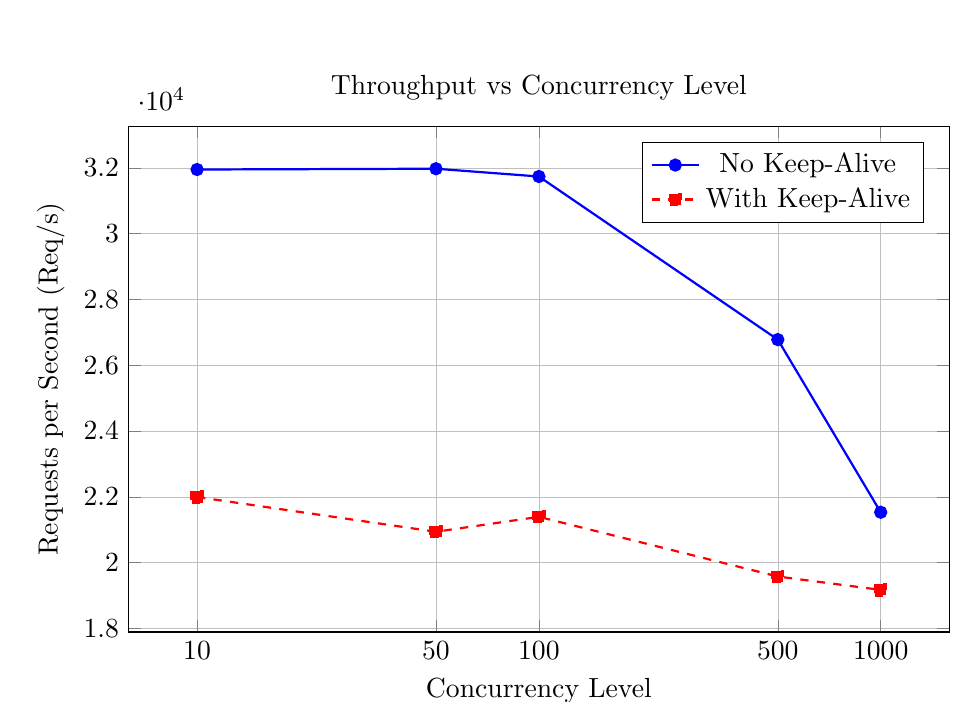
\begin{tikzpicture}
\begin{axis}[
    width=12cm,
    height=8cm,
    xlabel={Concurrency Level},
    ylabel={Requests per Second (Req/s)},
    xmode=log,
    log basis x={10},
    xtick={10,50,100,500,1000},
    xticklabels={10,50,100,500,1000},
    legend pos=north east,
    grid=both,
    grid style={line width=.1pt, draw=gray!20},
    major grid style={line width=.2pt,draw=gray!50},
    title={Throughput vs Concurrency Level}
]
\addplot[color=blue,mark=*,thick] coordinates {
    (10, 31948.41)
    (50, 31971.78)
    (100, 31735.84)
    (500, 26778.31)
    (1000, 21530.65)
};
\addlegendentry{No Keep-Alive}

\addplot[color=red,mark=square*,thick,dashed] coordinates {
    (10, 21994.49)
    (50, 20937.88)
    (100, 21391.65)
    (500, 19577.23)
    (1000, 19171.07)
};
\addlegendentry{With Keep-Alive}
\end{axis}
\end{tikzpicture}
\caption{Throughput performance comparison across different concurrency levels}
\end{figure}

\subsection{Results: Latency}
The following table presents the average latency per request (in milliseconds) measured under different concurrency levels.

\begin{table}[H]
\centering
\begin{tabular}{|c|c|c|}
\hline
\textbf{Concurrency} & \textbf{Latency (No Keep-Alive)} & \textbf{Latency (With Keep-Alive)} \\ \hline
10  & 0.313 ms & 0.455 ms \\ \hline
50 & 1.564 ms & 2.388 ms \\ \hline
100 & 3.151 ms & 4.675 ms \\ \hline
500 & 18.672 ms & 25.540 ms \\ \hline
1000 & 46.445 ms & 52.162 ms \\ \hline
\end{tabular}
\caption{Average latency comparison under different concurrency levels}
\end{table}

\begin{figure}[H]
\centering
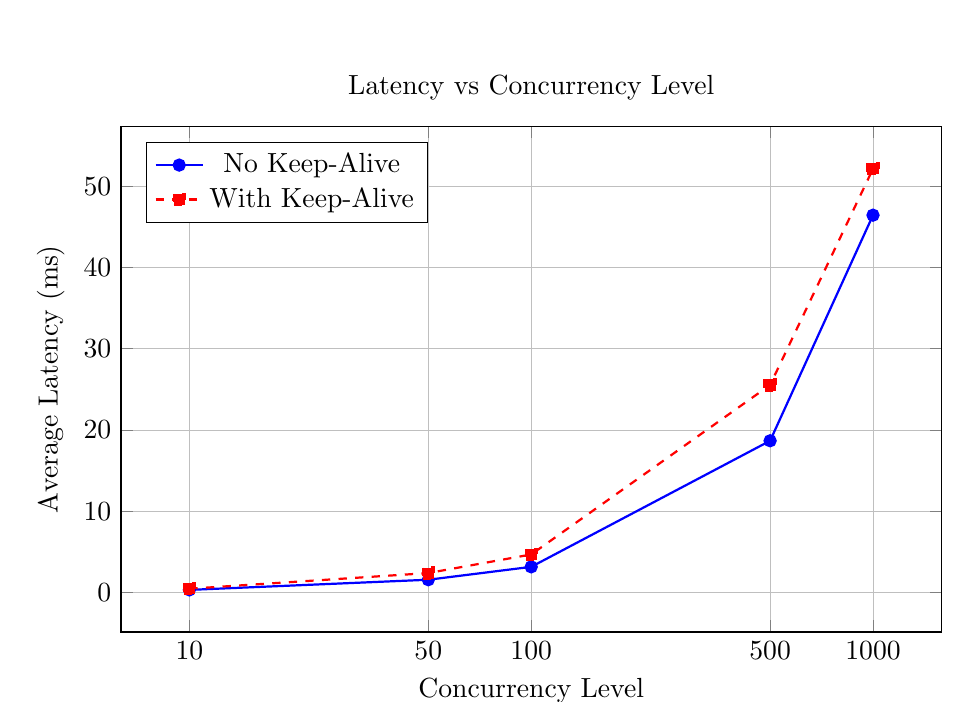
\begin{tikzpicture}
\begin{axis}[
    width=12cm,
    height=8cm,
    xlabel={Concurrency Level},
    ylabel={Average Latency (ms)},
    xmode=log,
    log basis x={10},
    xtick={10,50,100,500,1000},
    xticklabels={10,50,100,500,1000},
    legend pos=north west,
    grid=both,
    grid style={line width=.1pt, draw=gray!20},
    major grid style={line width=.2pt,draw=gray!50},
    title={Latency vs Concurrency Level}
]
\addplot[color=blue,mark=*,thick] coordinates {
    (10, 0.313)
    (50, 1.564)
    (100, 3.151)
    (500, 18.672)
    (1000, 46.445)
};
\addlegendentry{No Keep-Alive}

\addplot[color=red,mark=square*,thick,dashed] coordinates {
    (10, 0.455)
    (50, 2.388)
    (100, 4.675)
    (500, 25.540)
    (1000, 52.162)
};
\addlegendentry{With Keep-Alive}
\end{axis}
\end{tikzpicture}
\caption{Latency performance comparison across different concurrency levels}
\end{figure}

\subsection{Discussion of Results}

\paragraph{Throughput Analysis.}
The server demonstrates a good performance, reaching over 31,000 requests per second at low concurrency levels (10-100 concurrent clients) without keep-alive connections.

As concurrency increases beyond 500 clients, throughput gradually decreases because of switching overhead and queue contention. 

\paragraph{Latency Behavior.}
Latency scales approximately linearly with concurrency, which is expected behavior for a queuing system. At low concurrency (10 clients), the average response time is under 0.5ms, even at concurrency levels (1000 clients), latency remains under 55ms.

\paragraph{Keep-Alive Trade-offs.}
Interestingly, the benchmarks show that non-keep-alive connections achieve higher throughput in these tests. This is because Apache Bench with keep-alive (-k flag) maintains persistent connections, which can lead to head-of-line blocking in our architecture.

% ----------------------------------------------------------------------
% 6. Conclusion
% ----------------------------------------------------------------------
\section{Conclusion}

This project successfully achieved the implementation of a concurrent HTTP web server in C.
We combined the isolation benefits of multi-processing with the efficiency of multi-threading.

\paragraph{Achievements and Compliance.}
The server meets all mandatory requirements proposed in the proposal.
It handles static file serving, enforces synchronization using \textbf{POSIX Semaphores} and \textbf{Mutexes}, and guarantees data consistency across shared memory regions.
Testing with \texttt{ApacheBench} and \texttt{Valgrind} confirmed the system's stability under load, proving the absence of deadlocks, race conditions, and memory leaks.

\paragraph{Advanced Features.}
Going beyond the basic specifications, the system integrates advanced features found in production-grade servers.
The implementation of \textbf{HTTP Keep-Alive} and \textbf{Range Requests} improves the experience for persistent browsing and media streaming.
Furthermore, the \textbf{Real-time Web Dashboard} demonstrates the versatility of the shared memory architecture.

In conclusion, this project provided deep insights into system programming, particularly in the areas of IPC, concurrency control, and network protocol implementation.
\end{document}

